\scanpage{30}
\figure{\begin{tikzpicture}[scale=.82]
\draw (3.2,6.6) ellipse (2.25 and 1.9);
\draw (3.15,6.58) ellipse (2.32 and 1.96);
\draw (1.6,7.0) .. controls (4.1,9.2) and (5.0,8.2) .. (2.1,6.5) .. controls (1.0,5.7) and (4.8,8.1) .. (4.2,7.4) .. controls (3.6,6.5) and (1.8,5.5) .. (2.9,5.9) .. controls (5.7,7.5) and (4.6,6.3) .. (3.2,5.6) .. controls (2.2,4.7) and (5.9,7.0) .. (4.9,5.8) .. controls (3.6,4.4) and (4.1,5.3) .. (5.0,5.8);
\draw (3.5,6.7) ellipse (.32 and .38);\fill (3.47,6.7) circle (.025);
\node at (3.55,6.68) {$V$};\node at (3.94,6.94) {$U$};
\node at (1.5,8.55) {$\unsure{\phi_m}$};\node at (3.0,7.65) {$\unsure{\phi_n}$};
\node at (5.8,8.3) {$C^1$};\node at (7.2,7.2) {$\unsure{C^{n}}$};
\node[draw,ellipse] at (9.05,8.35) {$C^0$};\node at (10.4,8.3) {$\unsure{\Phi}$};
\draw (11.2,6.15) ellipse (.68 and .53);\draw (11.18,6.1) ellipse (.73 and .42);
\draw[->] (11.85,6.2)--(10.35,6.15);\draw (10.4,6.13)--(11.7,6.05)--(10.5,6.2);
\draw (5.45,6.95).. controls (8,6.8) and (9.6,5.9)..(11.6,6.35);
\draw[->] (8.7,4.9).. controls (8.0,5.6) and (6.1,6.3)..(4.95,6.25);
\draw (6.5,2.6).. controls (7.8,5.0) and (9.8,6.0)..(11.65,6.35);
\draw (12.95,7.1).. controls (12.4,6.1) and (12.5,5.3)..(13.05,4.6);
\node at (12.15,5.15) {$\unsure{m^1}$};\node at (6.4,4.9) {$\unsure{m-n}$};
\draw[->] (3.5,6.3)--(3.4,3.6);\node at (3.1,4.55) {$\sigma$};
\draw (3.7,3.9)--(3.7,2.8)--(5.0,2.35);\draw (3.7,2.8)--(2.2,1.5);
\draw (2.5,1.65)--(4.2,2.5);\draw (2.6,1.45)--(4.3,2.3);\draw (2.8,1.3)--(4.35,2.1);
\node at (4.15,3.75) {$R^{\unsure{m}}$};\node at (4.1,1.5) {$R^{\unsure{n}}$};
\draw (.4,2.2).. controls (.1,3.1) and (1.0,3.8)..(2.0,4.1);
\draw (.3,3.35)--(.65,2.4);\draw (.65,3.7)--(.95,2.65);\draw (1.0,4.0)--(1.3,3.05);\draw (1.3,4.0)--(1.6,3.25);
\draw (9.4,2.8) ellipse (3.8 and 1.7);\draw (9.7,3.4) ellipse (2.65 and .8);
\node at (9.65,3.4) {$\sigma(V)=\sigma(U)\cap R^n$};
\node at (8.75,2.2) {$A_0=\{(\sigma_i,(U_i,V_i))\}$};\node at (12.0,2.3) {$C^n$};
\draw (8.6,2.2) ellipse (3.0 and .8);
\end{tikzpicture}}

\figure{\begin{tikzpicture}\node[draw,ellipse,inner xsep=15pt,inner ysep=6pt] {$1)$ Familles connexes $C^r$, $r\geq0$};\end{tikzpicture}}
\[V_i\subset U_i\]
$2)$ Familles régulières (quasi-régulières), $C^r$, $r\geq1$
\[
\left.\begin{array}{ll}
3)\ \text{Familles naturelles},&r\geq1\\
4)\ \text{Familles normales},&r\geq1
\end{array}\right\}\ C^{r-1}
\]
\figure{
\begin{tikzpicture}\draw (0,0)--(10,.2);\end{tikzpicture}}
\figure{\begin{tikzpicture}\node[draw,ellipse,inner sep=8pt] {$(\sigma_1,(U_1,V_1))\qquad(\sigma_2,(U_2,V_2))$};\end{tikzpicture}}

$1)$ $V_1\cap V_2\ne\varnothing$

$2)$ $(\sigma'_1,(U_1\cap U_2,V_1\cap V_2))$

\hspace{2em}$(\sigma'_2,(U_1\cap U_2,V_1\cap V_2))$

\figure{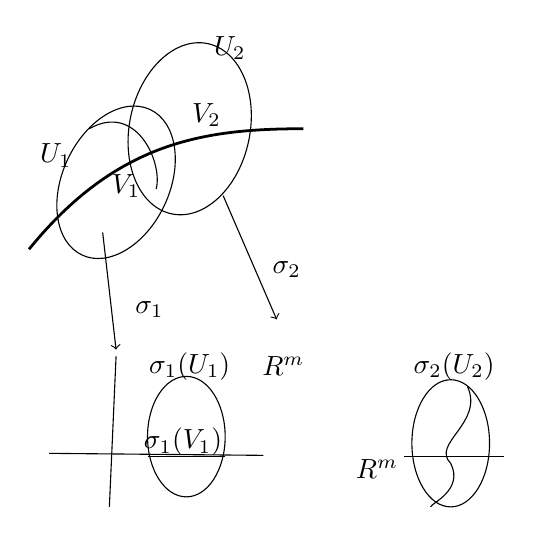
\begin{tikzpicture}[scale=.85]
\draw[rotate around={-25:(3,5.4)}] (3,5.4) ellipse (.8 and 1.2);
\draw[rotate around={-12:(4.1,6.2)}] (4.1,6.2) ellipse (.9 and 1.3);
\draw[line width=1pt] (1.7,4.4).. controls (3.0,6.0) and (4.3,6.2)..(5.8,6.2);
\draw (2.6,6.2)..controls (3.3,6.6) and (3.7,5.7)..(3.6,5.3);
\node at (2.1,5.8) {$U_1$};\node at (4.7,7.4) {$U_2$};\node at (3.15,5.35) {$V_1$};\node at (4.35,6.4) {$V_2$};
\draw[->] (2.8,4.65)--(3.0,2.9);\node at (3.5,3.5) {$\sigma_1$};
\draw[->] (4.6,5.2)--(5.4,3.35);\node at (5.55,4.1) {$\sigma_2$};
\draw (3.0,2.8)--(2.9,.55);\draw (2.0,1.35)--(5.2,1.32);
\draw (4.05,1.6) ellipse (.58 and .9);\draw (3.47,1.3)--(4.63,1.3);
\node at (4.1,2.65) {$\sigma_1(U_1)$};\node at (4.0,1.52) {$\sigma_1(V_1)$};\node at (5.5,2.65) {$R^m$};
\draw (7.3,1.3)--(8.8,1.3);\draw (8.0,1.5) ellipse (.58 and .95);
\draw (8.25,2.35)..controls (8.5,1.8) and (7.7,1.5)..(8.0,1.2)..controls (8.2,.8) and (7.7,.6)..(7.7,.55);
\node at (8.05,2.65) {$\sigma_2(U_2)$};\node at (6.9,1.12) {$R^m$};
\end{tikzpicture}}
\figure{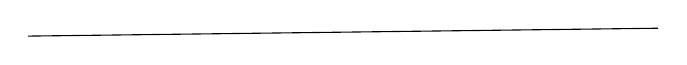
\begin{tikzpicture}\draw (0,0)--(8,.1);\end{tikzpicture}}
\[
U_1\cap V_2=V_1\cap V_2
\]
\[
U_2\cap V_1=V_1\cap V_2
\]
\mspage{29}
